% =====================================================================
% Șablon de raport pentru proiectul SADA (8-12 pagini fără anexe, A4, 11 pt).
% Overleaf: arhivați folderul latex/ și încărcați-l (New Project > Upload Project);
%           acolo IEEEtran există și șablonul arată ca un articol IEEE.
% Local:    latexmk -pdf main.tex  (fără IEEEtran instalat se folosește article).
% Figurile și tabelele se iau direct din ../../results/, generate de
% scripts/make_figures.py; pe Overleaf copiați-le în latex/figuri/.
% =====================================================================
\IfFileExists{IEEEtran.cls}
  {\documentclass[conference,a4paper,11pt]{IEEEtran}}
  {\documentclass[a4paper,twocolumn,11pt]{article}\usepackage[margin=1.8cm]{geometry}}
\usepackage[utf8]{inputenc}
\usepackage[T1]{fontenc}
\IfFileExists{romanian.ldf}{\usepackage[romanian]{babel}}{\usepackage{babel}\babelprovide[import,main]{romanian}}
\usepackage{graphicx,booktabs,amsmath,xcolor}
\usepackage{tikz}
\usetikzlibrary{arrows.meta,positioning,calc}
\usepackage{cite}
\usepackage[hidelinks]{hyperref}

% figură din results/ dacă există, altfel un chenar cu numele fișierului
\newcommand{\figsau}[2]{%
  \IfFileExists{../../results/figures/#1.pdf}{\includegraphics[width=#2]{../../results/figures/#1.pdf}}{%
  \IfFileExists{figuri/#1.pdf}{\includegraphics[width=#2]{figuri/#1.pdf}}{%
  \fbox{\parbox{0.9#2}{\centering\small\vspace{2em}Figura \texttt{\detokenize{#1}.pdf} lipsește:\\rulați \texttt{scripts/make\_figures.py}\vspace{2em}}}}}}

\begin{document}

\title{Recuperare ierarhică la defecte într-o rețea rutieră}
\author{Nume Prenume, Nume Prenume\\
Facultatea de Automatică și Calculatoare, Universitatea Politehnica Timișoara\\
\texttt{prenume.nume@student.upt.ro}}
\maketitle

\begin{abstract}
% 150-200 de cuvinte: problema, metoda, cel puțin un rezultat numeric, ce înseamnă.
% Îl scrieți ultimul.
Problema în două propoziții. Ce ați construit. Cum ați testat. Rezultatul principal,
cu un număr (de exemplu: „controllerul reduce ... cu X\,\% față de varianta fixă,
pe 20 de rulări''). Ce înseamnă rezultatul.
\end{abstract}

\noindent\textbf{Cuvinte cheie:} sisteme autoadaptive, MAPE-K, ...

\section{Introducere}
% aprox. 1 pagină: context, ce lipsește, obiectiv, contribuții verificabile.
Contextul și motivația \cite{albert2000,holme2002}.

Contribuțiile lucrării sunt:
\begin{itemize}
  \item ...
  \item ...
\end{itemize}

\section{Lucrări conexe}
% 1-1,5 pagini, minimum 6 referințe, cel puțin 2 din GECCO, AHS, ICES, ALife sau ECAL.
% Grupate pe idei; fiecare grup se încheie cu ce face lucrarea voastră diferit.
\subsection{...}
\subsection{Sisteme autoadaptive}
Bucla MAPE-K \cite{kephart2003} ... \cite{salehie2009}.

\section{Sistemul propus}
% 2-3 pagini: modelul, algoritmii, diagrama MAPE-K, parametrii și justificarea lor.
\subsection{Modelul}
\subsection{Bucla de adaptare}
Fig.~\ref{fig:mapek} prezintă bucla MAPE-K a sistemului.

\begin{figure}[t]
\centering
\resizebox{\columnwidth}{!}{%
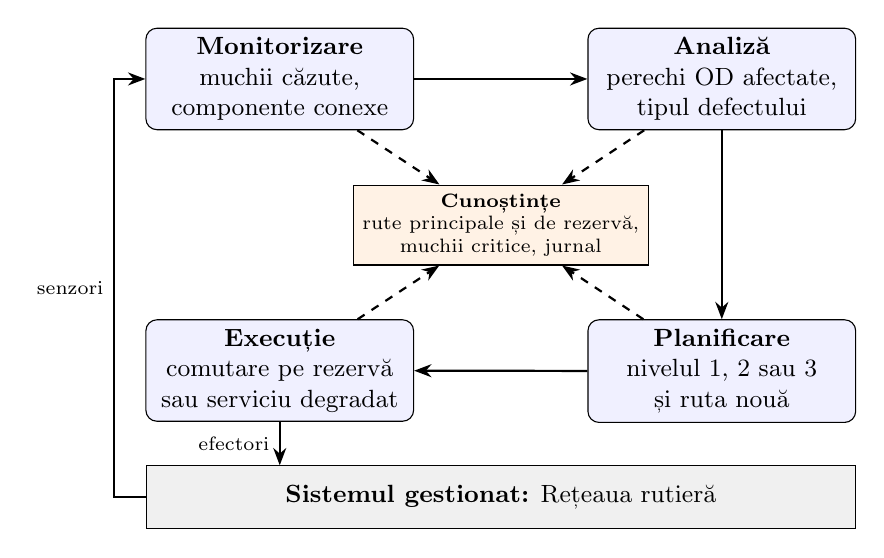
\begin{tikzpicture}[
  bloc/.style={draw, rounded corners, fill=blue!6, align=center, font=\small, minimum width=3.4cm, minimum height=1.25cm},
  kb/.style={draw, fill=orange!10, align=center, font=\scriptsize, minimum width=3.0cm, minimum height=0.9cm},
  sis/.style={draw, fill=gray!12, align=center, font=\small, minimum width=9cm, minimum height=0.8cm},
  sag/.style={-{Stealth[length=2.2mm]}, thick}]
  \node[bloc] (M) {\textbf{Monitorizare}\\muchii căzute,\\componente conexe};
  \node[bloc, right=2.2cm of M] (A) {\textbf{Analiză}\\perechi OD afectate,\\tipul defectului};
  \node[bloc, below=2.4cm of A] (P) {\textbf{Planificare}\\nivelul 1, 2 sau 3\\și ruta nouă};
  \node[bloc, below=2.4cm of M] (E) {\textbf{Execuție}\\comutare pe rezervă\\sau serviciu degradat};
  \node[kb] at ($(M)!0.5!(P)$) (K) {\textbf{Cunoștințe}\\rute principale și de rezervă,\\muchii critice, jurnal};
  \node[sis, below=1.2cm of $(E)!0.5!(P)$] (S) {\textbf{Sistemul gestionat:} Rețeaua rutieră};
  \draw[sag] (M) -- (A);
  \draw[sag] (A) -- (P);
  \draw[sag] (P) -- (E);
  \draw[sag, dashed] (M) -- (K); \draw[sag, dashed] (A) -- (K);
  \draw[sag, dashed] (P) -- (K); \draw[sag, dashed] (E) -- (K);
  \draw[sag] (S.west) -| node[pos=0.75, left, font=\scriptsize]{senzori} ([xshift=-0.4cm]M.west) -- (M.west);
  \draw[sag] (E.south) -- node[left, font=\scriptsize]{efectori} (E.south |- S.north);
\end{tikzpicture}}
\caption{Bucla MAPE-K a sistemului propus. Înlocuiți textele cu valorile concrete din proiect.}
\label{fig:mapek}
\end{figure}

\subsection{Parametrii}
\begin{table}[t]
\centering
\caption{Parametrii principali și justificarea lor}
\label{tab:param}
\small
\begin{tabular}{@{}p{0.28\columnwidth}p{0.18\columnwidth}p{0.42\columnwidth}@{}}
\toprule
Parametru & Valoare & Justificare \\
\midrule
... & ... & din literatură, din date sau dintr-un experiment preliminar \\
\bottomrule
\end{tabular}
\end{table}

\section{Date și configurare}
% aprox. 1 pagină: sursele datelor (cu licență), pregătirea lor, seed-uri, număr de rulări,
% perioada de încălzire, hardware, versiuni (requirements.lock.txt), comanda de rulare.

\section{Rezultate}
% 2-3 pagini. Comparație cu cel puțin o variantă de referință, medie ± abatere standard.
% Fiecare figură și fiecare tabel sunt comentate în text.
Tabelul~\ref{tab:rezultate} rezumă rezultatele pe toate scenariile.

\begin{table*}[t]
\centering
\caption{Rezultate (medie $\pm$ abatere standard pe $n$ rulări)}
\label{tab:rezultate}
\resizebox{\textwidth}{!}{%
\begin{tabular}{@{}llcccc@{}}
\toprule
Scenariu & Variantă & Perechi OD conectate [\%] & Creșterea costului mediu [\%] & Rute de rezervă folosite & Timp de recuperare [pași] \\
\midrule
\IfFileExists{../../results/tables/summary.tex}{\input{../../results/tables/summary.tex}}{%
\textit{rulați scripts/make\_figures.py} & \\}
\bottomrule
\end{tabular}}
\end{table*}

\begin{figure}[t]
\centering
\figsau{box_od_connected_pct}{\columnwidth}
\caption{Titlul spune ce se măsoară, pe ce scenarii, câte rulări.}
\label{fig:box}
\end{figure}

\section{Discuție și limite}
% aprox. 1 pagină: ce arată rezultatele, ce nu arată, ce ar trebui verificat în continuare.

\section{Concluzii}
% jumătate de pagină: ce s-a obținut (cu un număr) și ce rămâne deschis.

\IfFileExists{IEEEtran.bst}{\bibliographystyle{IEEEtran}}{\bibliographystyle{ieeetr}}
\bibliography{refs}

\appendix
\section*{Anexă: declarația privind instrumentele folosite}
\begin{tabular}{@{}p{0.25\columnwidth}p{0.65\columnwidth}@{}}
\toprule
Instrument & Pentru ce și în ce parte \\
\midrule
... & ... \\
\bottomrule
\end{tabular}

\noindent Comanda care reface rezultatele: \texttt{python scripts/run\_all.py \&\& python scripts/make\_figures.py}

\end{document}
